\documentclass[12pt,a4paper,DIV=calc]{scrartcl}
\usepackage[protrusion=true,expansion=true]{microtype}

\usepackage{float}
\usepackage{amssymb}
\usepackage[utf8]{inputenc}
\usepackage[T1]{fontenc}
\usepackage{graphicx}
\usepackage[bookmarks=true,hidelinks=true,breaklinks=true]{hyperref}
\usepackage{mathptmx}
\usepackage{cleveref}
\usepackage{enumitem}
\usepackage[backend=biber,natbib=true]{biblatex}
\usepackage[scaled=.92]{helvet}
\bibliography{references.bib}

\newtheorem{lemma1}{Lemma}

\begin{document}
\title{Seminar paper on Probabilistic Near-Duplicate Detection Using Simhash}
\author{Arne Beer, MN 6489196, University of Hamburg}
\date{08.07.2019}

\maketitle


\section{Introduction}

In the age of the modern Internet, many services depend in large parts on crawlers and proper document detection and duplication elimination, near duplicate document detection becomes a necessity.
Real time detection of which website has already been visited and whether a website is new or just has been edited are important tasks during crawling~\cite{paper:scaling_six_billion}.

Standard hashing functions are often inefficient and operate in $O(n^2)$ space requirements for RAM and computing time~\cite{book:hashing}.
At the same time, the size of available documents grow steadily.
Google's website index alone has multiple hundreds of billions of web pages and over 100 Petabyte in size, according to their information website~\cite{info:google_stats}.

This paper attends to the paper \emph{Seminar paper on Probabilistic Near-Duplicate Detection Using Simhash}~\cite{inproc:main}.
The main challenge tackled by this paper is to find all matching pairs of fingerprints withing a certain Hamming distance $h$.
At this time, the fasted implementation for this procedure has been \emph{Block-Permuted Hamming Search} (BPHS), which requires RAM space at least four times the size of the whole dataset.
The authors of~\cite{inproc:main} aim to design a new algorithm that allows significantly faster online and batch document comparison and furthermore reduces RAM requirements, in exchange for a small percentage of recall loss.

In the first chapters, the basics for understanding this topic will be explained.
Afterwards the proposed algorithm will be looked at and the authors' findings will be discussed.

\subsection{Conventional Hashing}

Hashing is a technique, which is used to map data of an arbitrary size to a fingerprint with some fixed size.
This procedure could be seen as a function  $f(i) \rightarrow j$, which produces a value $j$ from from any value $i$, where $j \in H$ and $H$ is the set of values of the fixed length $s$ with $s \in \mathbb{N}$.
Well-known hash functions are, for instance, \emph{MD5} or \emph{SHA265}.
These hashing functions are commonly used to check whether two files are absolutely identical or, for instance, to verify that a file has not been corrupted during transport.
This is possible, since these hashing functions are designed to flip half of the output hash bits on average, if an input bit changes~\cite{book:hashing}.
Without this property it would be easier to change the input without the hash signature being modified.
This would allow malicious third parties to, for instance, change code in a binary, without users being able to detect the change with the help of this hash and would require a full byte level comparison between the original and the copied file to verify its integrity.

If, on the other hand, one's goal is to find near duplicates, which are identical for the most part, but sometimes only differ by a few bits or bytes, this hashing approach immediately becomes useless, due to this property.
Due to the need for a hashing algorithm, that creates a fingerprint based on the features and structure of the input data, \emph{simhash} has been created.


\section{Simhash}

To compare documents for similarity a methodology to create some uniform value, which should be identical for two similar matching documents.

\emph{simhash} is a procedure used to create a fingerprint of a any kind of data.
This fingerprint can then be used to, for instance, inspect two files for similarity.

The process for creating such a fingerprint can completely differ depending on the features in the hashed data one is interested in.
In case one wants to find similar binary files, it would be reasonable to split the data into equal chunks and use these chunks as features.
For websites or documents, looking at the composition and structure of text could be a viable approach to select features for hashing
The original data can then be refined to a high dimensional vector of features.

\begin{figure}[H]
    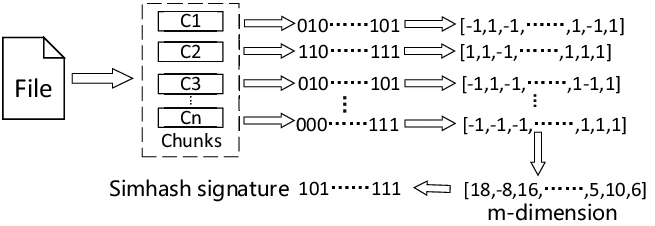
\includegraphics[scale=0.5]{./gfx/binary_chunk_fingerprint}
    \centering
    \caption{Visual example for calculating a \emph{simhash} fingerprint.
        A binary file split into chunks, which are then hashed.
    Combining all hashes results in the desired fingerprint.~\cite{article:sampling-similarity}}\label{fig:simhash-example}
\end{figure}

The size of available features can vary significantly and is completely in the hand of the designer for each \emph{simhash} implementation.
It's important to note, that there exists no clear guideline on which features of a data set are interesting and which features can be ignored.
The performance of a \emph{simhash} implementation thereby also depends on the chosen features and the respective properties of the dataset.
Such features can be for instance binary chunks, file extension~\cite{inproc:simhash}, individual words, tags or URLs~\cite{inproc:main}.

After determining in which way feature are extracted from the original data, each feature is hashed and mapped onto a fingerprint, which represents the constellation of features.

\begin{figure}[h]
    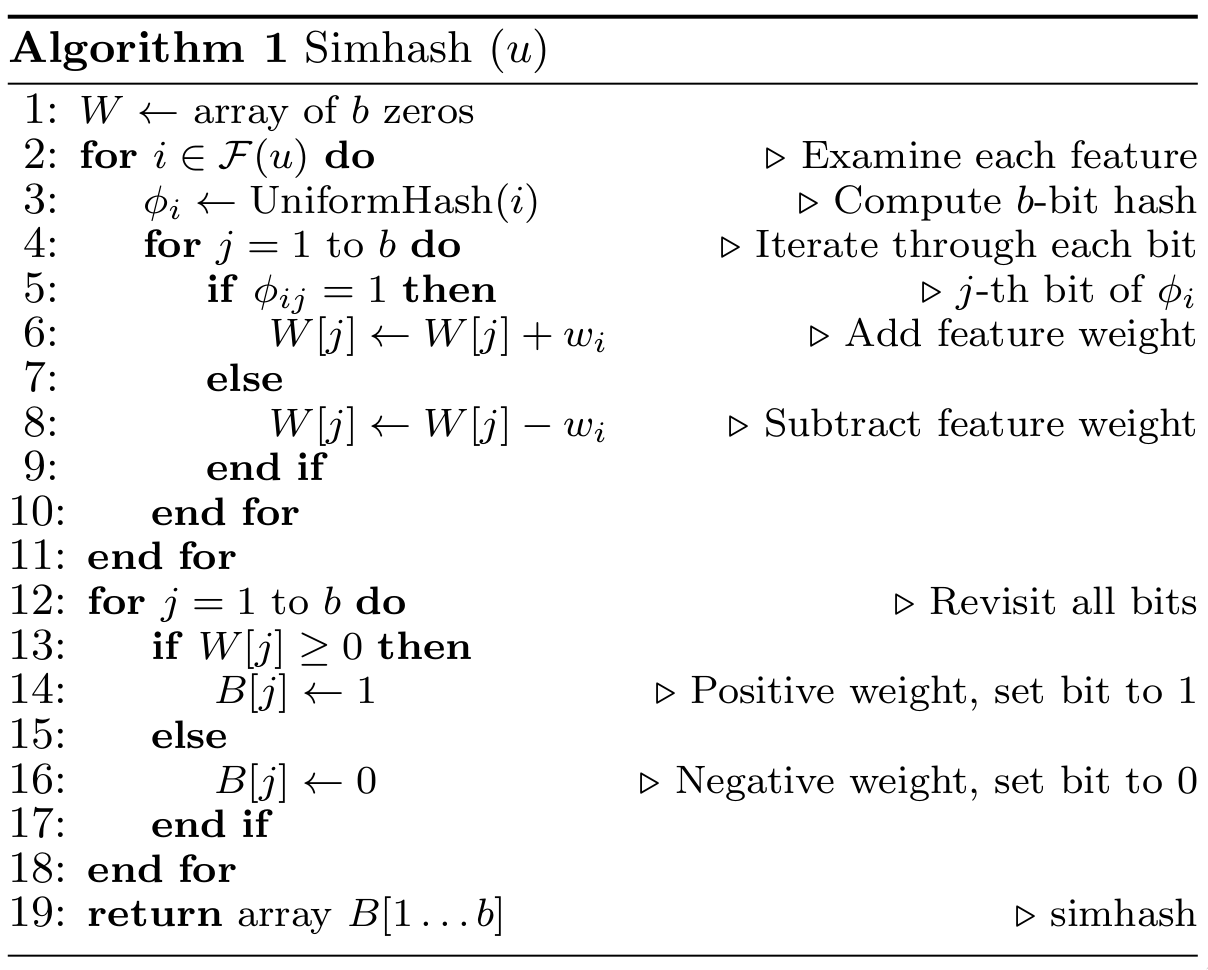
\includegraphics[scale=0.4]{./gfx/pseudocode.png}
    \centering
\end{figure}

Algorithm 1 explains the process of~\cite{inproc:evaluation} for creating fingerprints.
At first one iterates over the features subset $F(u)$ of size $b$, which is selected from the set $F$ of all unique features with $F(u) \in F$.
Each feature is then uniformly hashed to a fix size.
This uniform hashing can be seen as a random projection of a arbitrarily large feature to a fixed size.
The amount of ones and zeros in this hash are then counted.
A one increments the counter, a zero decrements it.
The result is then stored in a weight vector $W$ under the respective index of the feature. $W$ has the same length $b$.

After calculating all values of $W$, a new binary Vector $B$ will then be created with the same Length as $W$.
Each value $v$ with $v_i \geq 0$ at index $i$ will result in $B[i] = 1$, while each $v_i < 0$ will result in $B[i] = 0$.

\subsection{Weights and Hamming Distance}

To achieve their goal of decreasing the runtime of fingerprint comparisons, the authors of~\emph{inproc:main} investigated the properties and distribution of weights of the temporary weight vector $W$ that was introduced the previous section.

For their current work, they used normalized term frequency–inverse document frequency (TF-IDF) weights.
This kind of weights is used to reflect the importance of a word to a document in a collection and is great for text-based document comparison methods~\cite{Salton:1986:IMI:576628}.
The corpus of the researchers consisted of 70M web pages.

\begin{figure}[H]
    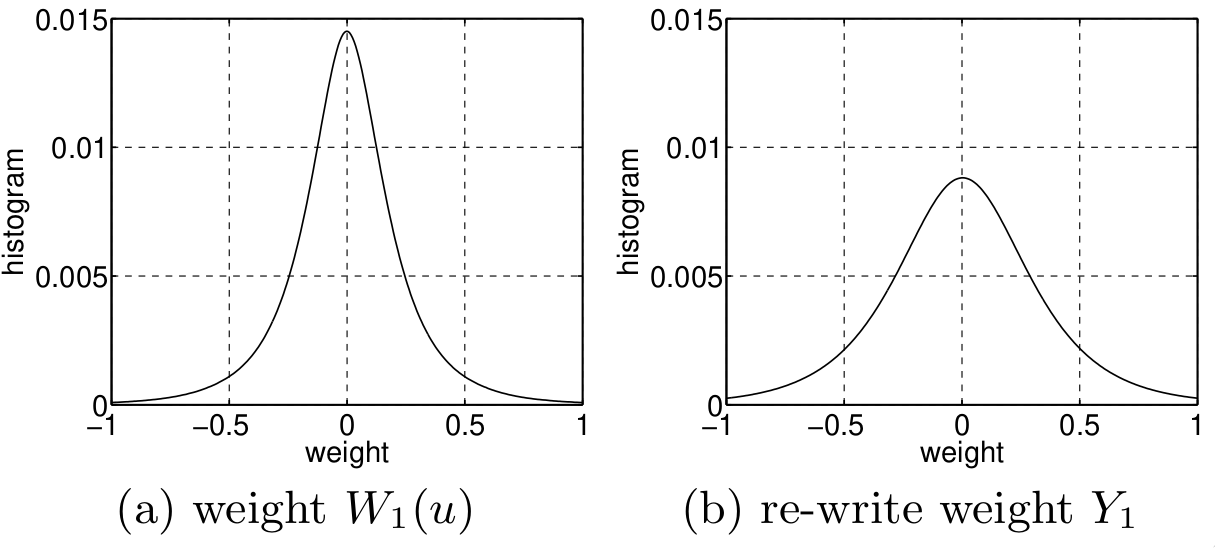
\includegraphics[scale=0.4]{./gfx/distribution.png}
    \centering
    \caption{Histogram of \emph{simhash} weights. A clear trend towards a Laplace-like distribution can be seen in (a).}\label{fig:weight-distribution}
\end{figure}

While using normalized TF-IDF weights, they noticed, that the distribution of weights rather resembles a Laplace-like distribution, than a Gaussian distribution, which has been expected, since the Central Limit theorem suggests it.
This can be seen in Figure~\ref{fig:weight-distribution}.

Using this knowledge they were able to generalize the formula for determining the specific weight of a feature to non-Bernoulli cases:

\[W_j(u) = \sum_{i \in F(u)} v_{ij}w_i(u)\]

$v$ is a vector, whose elements are drawn from a zero-mean symmetric distribution, which is theoretically equivalent to the Laplace-like distribution mentioned above.

After investigating the various probabilities and necessities for changing a weight to the side, it becomes apparent that certain bits are much more volatile to flip than others.
If one looks at the \emph{simhash} weights $(12, 0, -10)$, the second bit is much more likely to flip to the negative side, when small changes occur, than the other weights.
Much bigger changes would be needed to flip the weights at position 1 or 3.


\section{Bit order}

With the insight gained in the previous section, we are now able determine, which bits are more volatile to flip than others.
This knowledge can be utilized to determine an order, that should be used to determine the Hamming distance $h$ between the fingerprint and all hashes in the collection $D$.
While this is straight forward for single bit flips, where bits are simply ordered by their volatility, it becomes more complex, as soon as one wants to detect two-bit combination flips.

\subsection{Ordering}

$p_j(u)$ be the probability of another page in $D$, which has a flipped bit in position $j$ in the simhash of a page $u$ with $p_j(u) = P(Y_j > |W_j(u)|)$.
$Y$ is the random weight chance that occurs to changes in a document with $Y = X_j^{\alpha} - X_j^{\beta}$, where $X_j^{\alpha} - X_j^{\beta}$ are corresponding to the changed features.

Now it's possible to order and limit the Hamming search to the most likely subsets of hash bits.
For this let $S \subseteq \{1,2,\dots, b\}$ be a subset of non-empty hash bits.
The probability for the existence of a page in $D$ with differing bits on $S$ is then:

\[p(u,S) = \prod_{i \in S}p_i(u) \prod_{j \notin S}(1-p_j(u)) \]

Creating all possible subsets of $S$ in decreasing would be too time and space consuming, since it requires $\Theta(l \log l)$ operations and $\Theta(\sum_{i=1}^{h} ({b \atop i}))$ space.

\subsection{Volatility Heap}
To tackle the computation power and space requirement problems mentioned in the section above, the authors of~\cite{inproc:main} create a new data structure they call \emph{Volatility Ordered Set Heap} (VOSH).

For defining such a data structure, a specific property of the Sets of considered bits must be ensured.

\begin{lemma1}
If two sets $S_1, S_2$ of the same size $h$ differ in exactly 1 bit and $S_1 \prec S_2$, then $\forall u : p(u, S_1) \geq p(u, S_2)$.
\end{lemma1}

$\prec$ represents the lexicographical comparison operator on ${S}$. Lemma 1 describes that two sets fulfill $S_1 \prec S_2$, if there exists an index $i < h$ such that both sets have the same leading elements of length $i$, but $S_2$ is still larger in the $(i+1)$th element.


\begin{figure}[H]
    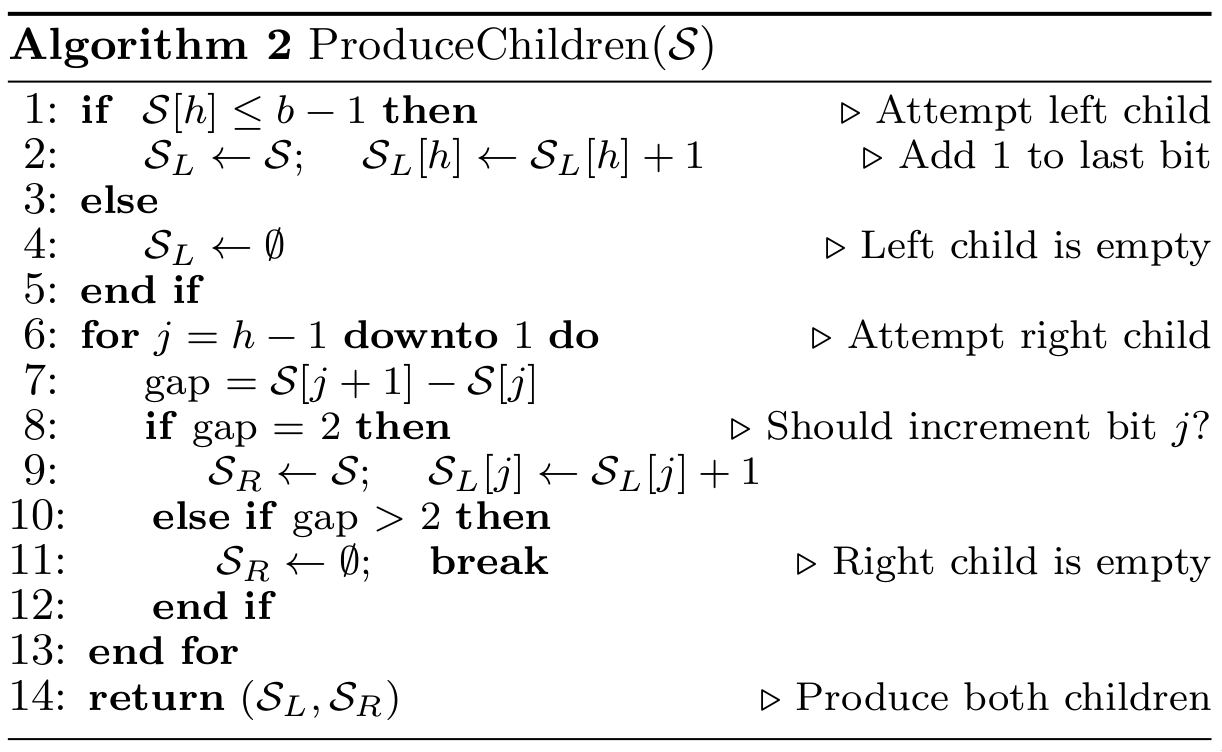
\includegraphics[scale=0.4]{./gfx/vosh_algorithm.png}
    \centering
    \caption{Pseudocode representation for the generation of a Volatility Ordered Set Heap (VOSH).}\label{fig:vosh-algorithm}
\end{figure}


\begin{figure}[H]
    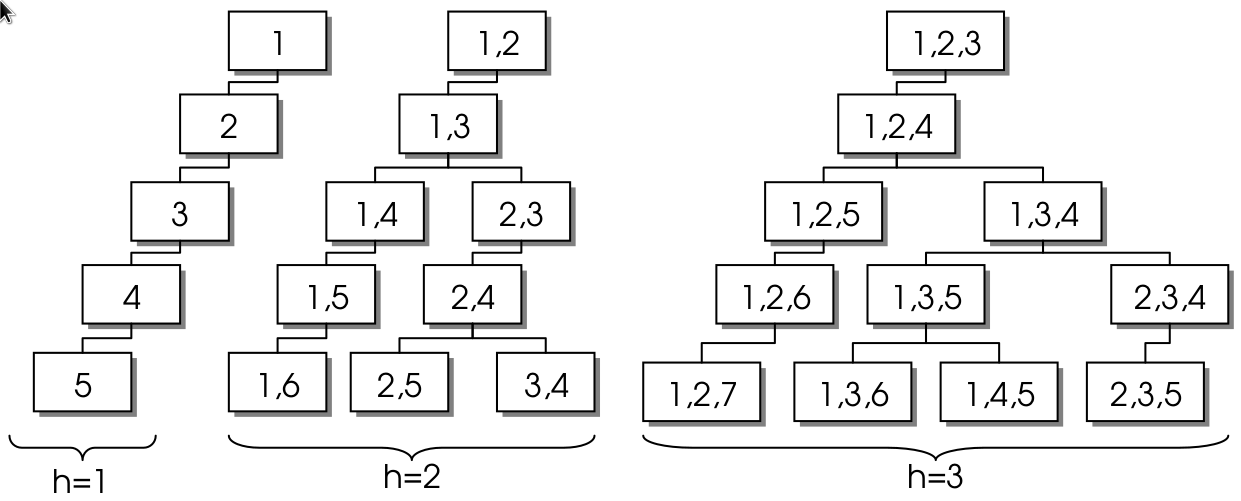
\includegraphics[scale=0.4]{./gfx/vosh_structure.png}
    \centering
    \caption{Example for a generated VOSH structure generated by Algorithm 2.}\label{fig:vosh-structure}
\end{figure}


The assertions gained by Lemma 1 allow us to create an algorithm, that creates a space efficient lookup data structure for determining near-duplicates within a certain Hamming distance $h$.
The bit combinations are sorted using the algorithm visualized in figure~\ref{fig:vosh-algorithm}.

The algorithm creates a binary tree structure, which is generated as follows.
For each node, check, whether the rightmost bit can be incremented.
If that is the case, create a new node with the new bit constellation as the left child node.
If the bit cannot be incremented, the left child node will be omitted.

At the same time, check the bits from right to left whether there exists a difference (or gap) between two adjacent bits that equals 2.
If there exists such a gap, the left bit of those two bits is incremented.
The new bit constellation now forms the right child node.
If there is no such gap, the right child node is simply omitted.

Figure~\ref{fig:vosh-structure} shows example results for volatility heaps created by this algorithm.
The volatility heaps are created with different Hamming distance thresholds $h$.

\subsection{Probabilistic Search}

While using VOSH for probabilistic search a new problems become apparent that have not been addressed yet.
VOSH is not and cannot be capable of deciding, which of two siblings at each level is more optimal.
To solve this problem, the authors of~\cite{inproc:main} introduce an additional data structure $M$, which is a max-heap operating on a key-value pairs.

\begin{figure}[H]
    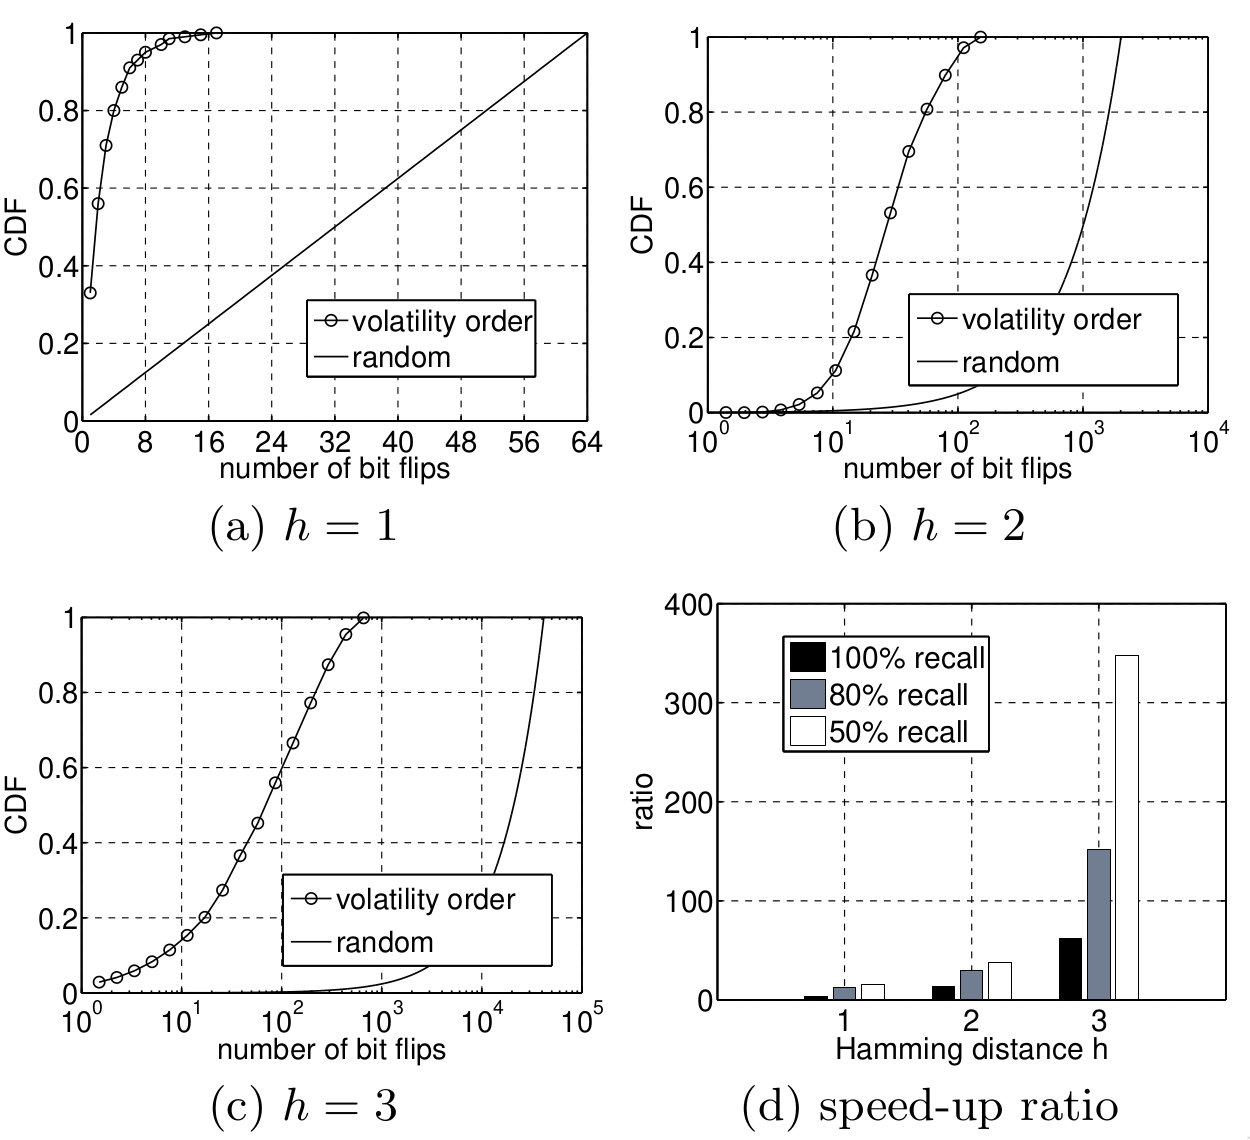
\includegraphics[scale=0.33]{./gfx/vosh-performance.png}
    \centering
    \caption{Performance results comparing random comparison search and volatility order based search.}\label{fig:vosh-performance}
\end{figure}

The key is the probability of flips in page $u$ for set $S$, while the value is the actual value $S$.
M is populated with tuples generated by the $h$ root nodes of VOSH trees.

Using this methodology they test their implementation on an 8B web page corpus, with 64 bit hashes and various Hamming distances.
They then create all hashes for their corpus and randomly select 8M random pairs of \emph{simhashes} and flip $h$ random bits on each pair.
The results of these tests can be seen in Figure~\ref{fig:vosh-performance}.

The authors compared their VOSH-algorithm to random hash comparison and were able to show that there exists significant speedup up to 61 times for 100\% recall and a hamming distance of 3 in Figure~\ref{fig:vosh-performance} (d).

It is notable, that the random approach needs 64 flips to get a 100\% recall for all hamming distances.
This is to be expected, but still shows how inefficient such an approach would be.

Also it becomes apparent that the speedup for VOSH in comparison to a random approach gets higher, the bigger the Hamming distance $h$ gets, making it viable for larger hash sizes with proportional small Hamming distances.


\subsection{Probabilistic Simhash Matching}

The VOSH algorithm is implemented in a framework called Probabilistic Simhash Matching (PSM).
PSM features an online mode, in which all existing Fingerprints are stored in a collection $H$.
$H$ is sorted before the algorithm start, therefore the cost for sorting the set are not considered here.

Since using VOSH on all bites and the whole dataset $H$ is highly inefficient only a small range of bits.
The search is then performed on a small range of uppermost bits, which are called headers.
For the purpose of performant header lookups a hash table of size $t$ is used as can be seen in Figure~\ref{fig:vosh-lookup}.

\begin{figure}[h]
    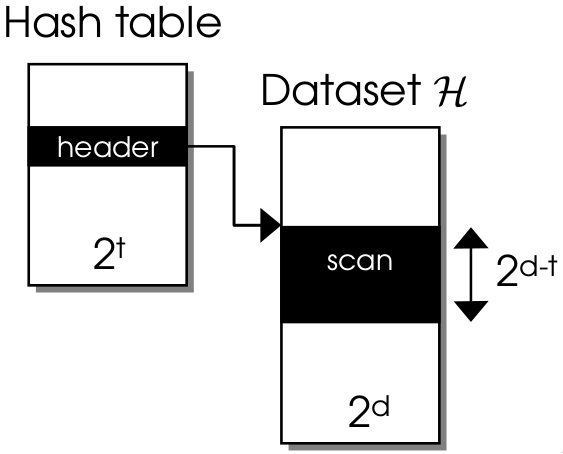
\includegraphics[scale=0.33]{./gfx/vosh-online.png}
    \centering
    \caption{The lookup using PSM is not performed on the whole dataset $H$, but rather on a small subset of bits defined by the header in the hash table.}\label{fig:vosh-lookup}
\end{figure}


The algorithm also features a batch query mode, which accumulates new fingerprints in a set $Q$, until it reaches size $m$.
Once the threshold is reached, PSM splits the existing collection in chunks of $m$ fingerprints and matches each $x \in Q$ against the loaded chunk.
Afterwards all $x \in Q$ are sorted and appended to the existing collection.


\section{Conclusion}
The authors of~\cite{inproc:main} compare their proposed methodology to the, at their time, most performant implementation, namely Block-Permuted Hamming Search (BPHS), for finding similar \emph{simhashes} in a document collection~\cite{Manku:2007:DNW:1242572.1242592}.

\begin{figure}[H]
    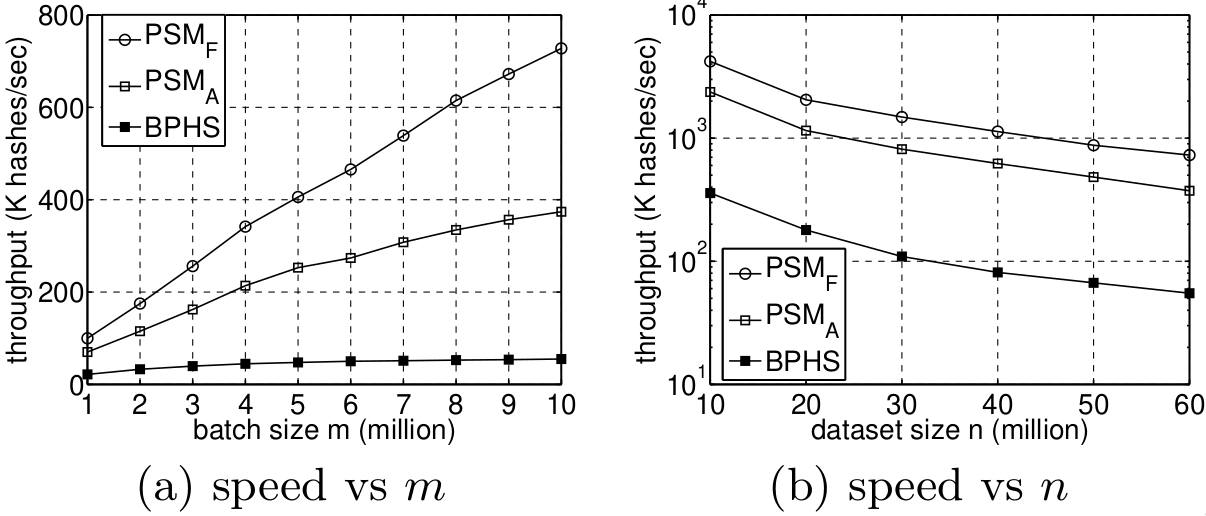
\includegraphics[scale=0.4]{./gfx/performance_comparison.png}
    \centering
    \caption{Performance comparison between PSM and BPHS in batch mode.}\label{fig:performance-comparison}
\end{figure}

PSM outperforms BPHS in pretty much every scenario, by sacrificing a very small amount of recall.
This new approach can be seen as a viable addition for \emph{simhashing} algorithms.


\section{Impact in the scientific community}
This paper has been cited by 36 different publications.
Considering this paper has been released 2011, it's still cited by papers and books in 2019, which makes it still valuable contribution to the scientific community.

\section{Relevance as of 2019}
Near duplicate detection is still a very important research field.
The current trend shows, that data will continue to be generated in a exponential manner.
Tackling an even larger amount of data and filtering it for duplicates will continue to create new challenges in respect to data throughput and RAM limitations.

Simhash is being used by many companies in various application fields.
For instance, Google started using \emph{simhash} in 2007 for their web-crawling services~\cite{Manku:2007:DNW:1242572.1242592}.
With Google being one of the biggest Internet companies and the number one search engine, relevance of this topic is obviously very high.

This is especially interesting, since this paper takes the original algorithm proposed for usage in Googles web crawler~\cite{Manku:2007:DNW:1242572.1242592} as comparison for their own research while showing that they are capable of significantly speeding up the lookup.

\printbibliography
\end{document}
